
\subsection*{1.}

On a \(p(T) = 0{,}30\) et \(p_T(C) = 0{,}60\).

\subsection*{2.}

\begin{center}
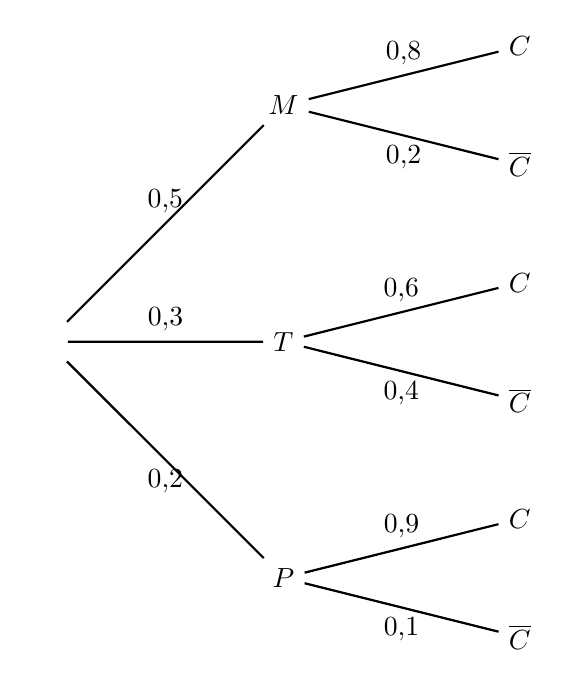
\begin{tikzpicture}[thick, scale=1.5] %{,} ,sloped
\node (P_-1_0) at (-2,-2.5) {$\phantom{A}$};
\node (P_0_0) at (0,-0.5) {$M$};
\draw (P_-1_0) -- (P_0_0) node[midway, above] {$0{,}5$};
\node (P_1_0) at (2,-0) {$C$};
\draw (P_0_0) -- (P_1_0) node[midway, above] {$0{,}8$};
\node (P_1_1) at (2,-1) {$\overline{C}$};
\draw (P_0_0) -- (P_1_1) node[midway, below] {$0{,}2$};
\node (P_0_2) at (0,-2.5) {$T$};
\draw (P_-1_0) -- (P_0_2) node[midway, above] {$0{,}3$};
\node (P_1_2) at (2,-2) {$C$};
\draw (P_0_2) -- (P_1_2) node[midway, above] {$0{,}6$};
\node (P_1_3) at (2,-3) {$\overline{C}$};
\draw (P_0_2) -- (P_1_3) node[midway, below] {$0{,}4$};
\node (P_0_4) at (0,-4.5) {$P$};
\draw (P_-1_0) -- (P_0_4) node[midway, below] {$0{,}2$};
\node (P_1_4) at (2,-4) {$C$};
\draw (P_0_4) -- (P_1_4) node[midway, above] {$0{,}9$};
\node (P_1_5) at (2,-5) {$\overline{C}$};
\draw (P_0_4) -- (P_1_5) node[midway, below] {$0{,}1$};
\end{tikzpicture}
\end{center}

\subsection*{3.}

\paragraph{a.} \(M \cap C\) représente l'événement : « le client a pris des macarons et un café ».
\[
p(M \cap C) = p(M) \times p_M(C) = 0{,}5 \times 0{,}8 = 0{,}4.
\]

\paragraph{b.} On a de même :
\[
p(T \cap C) = p(T) \times p_T(C) = 0{,}3 \times 0{,}6 = 0{,}18
\]
\[
p(P \cap C) = p(P) \times p_P(C) = 0{,}2 \times 0{,}9 = 0{,}18
\]

D'après la loi des probabilités totales :
\begin{align*}
p(C) &= p(M \cap C) + p(T \cap C) + p(P \cap C) \\
&= 0{,}4 + 0{,}18 + 0{,}18 = 0{,}76.
\end{align*}

\subsection*{4.}

Il faut calculer :
\[
p_C(M) = \dfrac{p(C \cap M)}{p(C)} = \dfrac{0{,}4}{0{,}76} \approx 0{,}5263,
\]
soit \(0{,}53\) au centième près.

